% V3: control policy refiner with the solver as decoder (cost weights -> Riccati gains), up to 6 pages.
% Based on the IEEE conference template (IEEEtran, conference mode), with small deviations
% (author block with advisors, tighter floats).
\documentclass[conference]{IEEEtran}
\IEEEoverridecommandlockouts
\usepackage[T1]{fontenc}
\usepackage{cite}
\usepackage{amsmath,amssymb,amsfonts}
\usepackage{graphicx}
\usepackage{textcomp}
\usepackage{xcolor}
\usepackage{booktabs}
\usepackage{array}
\usepackage{url}
\usepackage{tikz}
\usetikzlibrary{arrows.meta,positioning,calc,fit}

\newcommand{\R}{\mathbb{R}}
\newcommand{\T}{^{\top}}
\newcommand{\mpc}{\mathrm{MPC}}
\newcommand{\xb}{\bar{x}}
\newcommand{\ub}{\bar{u}}
\setlength{\textfloatsep}{9pt plus 2pt minus 2pt}
\setlength{\dbltextfloatsep}{9pt plus 2pt minus 2pt}
\setlength{\abovecaptionskip}{3pt}
\raggedbottom

\begin{document}
\bstctlcite{IEEEexample:BSTcontrol}

\title{Control Policy Refiner in Legged Robotics:\\ Preliminary Results}

\author{\IEEEauthorblockN{Norawit Nangsue}
\IEEEauthorblockA{Advisors: Fumio Kanehiro}
\IEEEauthorblockA{University of Tsukuba, Ibaraki, Japan}
}

\maketitle

\begin{abstract}
A model predictive controller (MPC) based on differential dynamic programming drives a humanoid robot between two solves with a feedback policy made of a state set-point and a gain matrix.
This policy is optimal for the model, but not for the real-world robot.
We propose a \emph{control policy refiner} that corrects the gain and the set-point to make the system more robust to uncertainty.
Since the gain matrix is too large to learn directly, the refiner outputs a latent representation of cost-weight scales and a set-point shift.
Then, one Riccati backward pass along the current trajectory turns the scaled weights into a full gain matrix.
The gains that the refiner produces are therefore the optimal feedback of a local problem, and the set-point shift is designed to respect the contact constraints.
This keeps exploration structured and small.
For the base controller, we apply IS-MPC to provide the center of mass (CoM) and gait solution, and feed it as a reference to a lower-body MPC. The upper body is stabilized with a linear quadratic regulator (LQR).
In simulation, the base controller walks at up to 0.5\,m/s without falling on random command schedules and recovers 80 of 104 pushes over a full stride, on par with an open-source IS-MPC walker.
The refiner itself has not been trained yet.
\end{abstract}

\begin{IEEEkeywords}
humanoid robots, model predictive control, residual reinforcement learning, feedback gain modification, set-point modification
\end{IEEEkeywords}

\section{Introduction}

Model-based walking controllers for humanoid robots are commonly built in two layers.
The upper layer plans with a reduced model such as the linear inverted pendulum (LIPM) \cite{kajita2001lipm,kajita2003preview}, centroidal dynamics \cite{orin2013centroidal,dai2014centroidal}, or single rigid body dynamics \cite{dicarlo2018cheetah,winkler2018gait}.
The lower layer is a whole-body controller that computes the joint torques, often implemented as a quadratic programming (QP)-based controller \cite{saab2013dynamic,herzog2016momentum} or a model predictive controller (MPC) \cite{mastalli2020crocoddyl,dantec2022wbmpc}.

A reduced model is simple enough to analyze thoroughly, so a control law that keeps the robot walking without falling can be derived from it and computed fast.
A control law based on the LIPM adjusts the zero-moment point (ZMP) \cite{vukobratovic2004zmp} to control the center of mass (CoM) position. Recent approaches rather steer the CoM by manipulating the divergent component of motion (DCM) \cite{takenaka2009dcm,englsberger2011capture}, closely related to the capture point \cite{pratt2006capture,koolen2012capturability}, because the CoM always follows the DCM.
The DCM is the unstable part of the LIPM dynamics, and once the ZMP satisfies the boundedness condition \cite{lanari2014boundedness}, the DCM never grows indefinitely.
Intrinsically stable MPC (IS-MPC) \cite{scianca2020ismpc,dallard2025adios} applies the theory by using it as a constraint, leading to long-term robot balancing.

On the other hand, the whole-body controller only has to track the CoM, foot and contact references it receives.
This separation of concerns makes model-based walking fast enough for practical use.

However, any model-based controller is optimal only under its model assumptions; it does not take model mismatch and other uncertainties into account.
In contrast, learning-based controllers are trained in simulation with reinforcement learning (RL) \cite{hwangbo2019learning,lee2020learning,rudin2022minutes,radosavovic2024humanoid}. As a result, they can adapt to such effects from experience.
However, they are black boxes, which raises concerns about safety and explainability.

This opens a new landscape that embraces both approaches: residual reinforcement learning (ResRL) \cite{silver2018residual,johannink2019residual}. This technique learns a correction on top of a model-based controller by modifying a joint torque or a position target \cite{cheng2025rambo,jeon2025residualmpc}.

Instead of applying the residual to the output directly, this contribution proposes a way to adjust the control law.
When the optimal control problem is solved with differential dynamic programming (DDP) \cite{mayne1966ddp}, a closed-loop feedback policy is provided as a by-product for controlling the system in real time.
This policy consists of the Riccati gains and a set-point.

We aim to train a residual policy, the \emph{refiner}, over the gain and set-point of this closed-loop feedback controller, so that the integrated system becomes more robust to uncertainty.

Nevertheless, learning the gains directly is impractical. In our whole-body MPC, each Riccati gain maps the 36-dimensional state error of the floating base and the twelve leg joints, in position and velocity, to twelve joint torque commands, so a policy would have to learn $12\times36=432$ elements at every node.
To solve this problem, we propose that the refiner acts on the \emph{cost} instead: once DDP performs a single backward pass with the modified cost, the new gain is computed. Together with a set-point shift, this approach drastically reduces the learned variables to a latent representation $\gamma$ of 10 cost-weight scales for the gain and 12 shifts for the set-point, 22 numbers in total.

This paper presents the model-based controller in Section~\ref{sec:base}, the refiner in Section~\ref{sec:method}, and the simulation results of the model-based controller in Section~\ref{sec:results}.

\section{Related Work}

\emph{Gait generation with reduced models.}
Preview control \cite{kajita2003preview} and linear MPC gait generators \cite{wieber2006mpc}, which can also choose the footsteps \cite{herdt2010online}, are all based on the LIPM.
IS-MPC \cite{scianca2020ismpc} enforces the boundedness condition of \cite{lanari2014boundedness} as a constraint.
Dallard \emph{et al.} \cite{dallard2025adios} closed the loop on the measured state and added a pre-optimization of the footstep timing, which is essential for push recovery \cite{khadiv2020timing}.

\emph{Whole-body MPC and Riccati feedback.}
DDP \cite{mayne1966ddp,li2004ilqr,tassa2012synthesis} solves the whole-body problem fast enough for MPC and has been demonstrated on a torque-controlled humanoid \cite{dantec2022wbmpc}.
Its Riccati gains are a first-order approximation of how the MPC solution changes with the state \cite{dantec2022firstorder}, so they can run the feedback faster than the solver.
To be usable on hardware, they must be consistent with the contact constraints \cite{grandia2019feedback}.

\emph{RL combined with model-based control.}
A policy can imitate or track a model-based plan \cite{carius2020mpcnet,reske2021imitation,jenelten2024dtc,kang2023rlmodel}, plan footsteps for a model-based controller \cite{gangapurwala2022rloc}, or correct a model-based controller \cite{cheng2025rambo,jeon2025residualmpc}.
Closer to our approach, learning can set the parameters of an MPC \cite{hewing2020lbmpc}: the decision variables of a quadrotor MPC \cite{song2022policysearch}, a learned cost in a differentiable MPC \cite{amos2018diffmpc,romero2024acmpc}, or in theory any parameter of an MPC used as a policy \cite{gros2020nmpcrl}.
These methods solve the MPC again with the new parameters, which changes the planned motion.
Our refiner keeps the plan and changes only the reaction, decoding the weights into new gains with one backward pass between two solves.
The idea is close to variable impedance learning \cite{buchli2011variable} and LQR weight tuning \cite{marco2016lqr}, applied online to the time-varying gains of a whole-body MPC, which makes it more applicable to multi-joint robots that demand efficient computation.

\section{Model-based Controller}
\label{sec:base}

\begin{figure*}[t]
\centering
\resizebox{0.96\textwidth}{!}{%
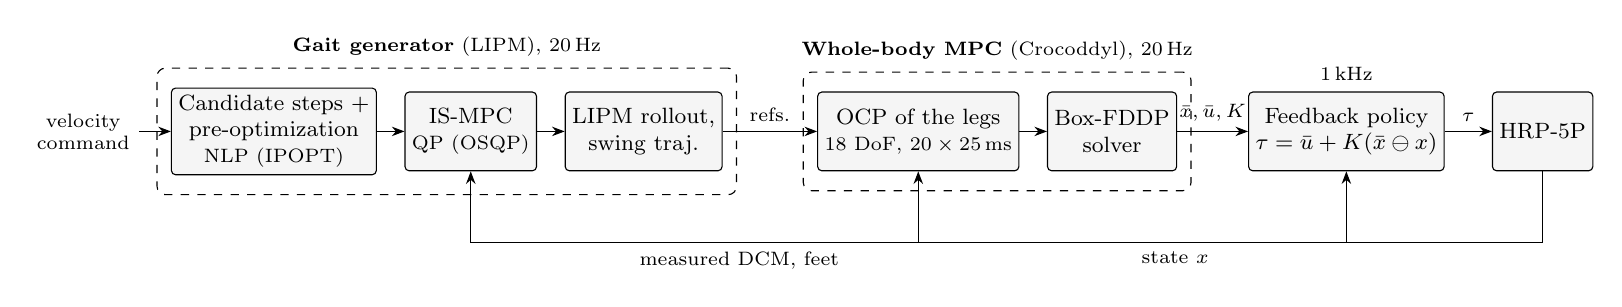
\begin{tikzpicture}[font=\footnotesize, >={Stealth[length=1.6mm]},
  blk/.style={draw, rounded corners=1.5pt, minimum height=10mm, align=center, inner sep=2.5pt, fill=black!4},
  grp/.style={draw, dashed, rounded corners=3pt, inner sep=5pt, inner ysep=7pt},
  lab/.style={font=\scriptsize, align=center}]
\node[lab] (cmd) {velocity\\command};
\node[blk, right=4mm of cmd] (ftpp) {Candidate steps +\\pre-optimization\\{\scriptsize NLP (IPOPT)}};
\node[blk, right=3.5mm of ftpp] (ismpc) {IS-MPC\\{\scriptsize QP (OSQP)}};
\node[blk, right=3.5mm of ismpc] (roll) {LIPM rollout,\\swing traj.};
\node[blk, right=12mm of roll] (ocp) {OCP of the legs\\{\scriptsize 18 DoF, $20\times25$\,ms}};
\node[blk, right=3.5mm of ocp] (ddp) {Box-FDDP\\solver};
\node[blk, right=9mm of ddp] (ric) {Feedback policy\\$\tau=\ub+K(\xb\ominus x)$};
\node[blk, right=6mm of ric] (rob) {HRP-5P};
\node[grp, fit=(ftpp)(ismpc)(roll)] (gg) {};
\node[grp, fit=(ocp)(ddp)] (wb) {};
\node[lab, above=0.2mm of gg.north] {\textbf{Gait generator} (LIPM), 20\,Hz};
\node[lab, above=0.2mm of wb.north] {\textbf{Whole-body MPC} (Crocoddyl), 20\,Hz};
\node[lab, above=0.2mm of ric.north] {1\,kHz};
\draw[->] (cmd) -- (ftpp);
\draw[->] (ftpp) -- (ismpc);
\draw[->] (ismpc) -- (roll);
\draw[->] (roll) -- node[lab, above] {refs.} (ocp);
\draw[->] (ocp) -- (ddp);
\draw[->] (ddp) -- node[lab, above] {$\xb,\ub,K$} (ric);
\draw[->] (ric) -- node[lab, above] {$\tau$} (rob);
\coordinate (fb) at ($(ric.south)+(0,-9mm)$);
\draw[->] (rob.south) |- (fb) -- (ric.south);
\draw[->] (fb) -| node[lab, pos=0.2, below] {state $x$} (ocp.south);
\draw[->] (fb -| ocp.south) -| node[lab, pos=0.2, below] {measured DCM, feet} (ismpc.south);
\end{tikzpicture}}
\caption{Base controller. An IS-MPC gait generator sends CoM, foot and contact references to a whole-body MPC built on Crocoddyl. The feedback policy of the MPC runs at 1\,kHz on the HRP-5P model in MuJoCo.}
\label{fig:base}
\end{figure*}

\begin{figure}[t]
\centering
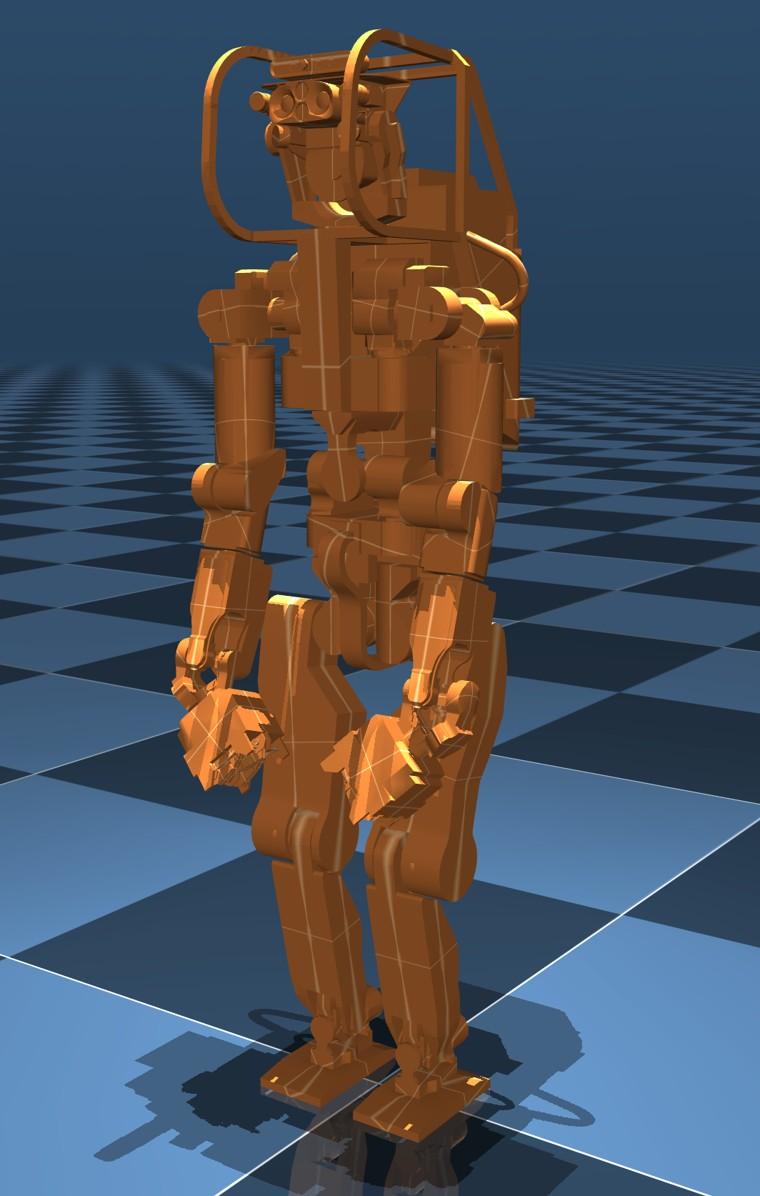
\includegraphics[width=0.42\columnwidth]{figures/hrp5p.jpg}
\caption{The HRP-5P model in MuJoCo. All runs start from this standing posture.}
\label{fig:robot}
\end{figure}

\subsection{CoM and Gait Controller}
For a constant CoM height $z_c$, let $c$ be the CoM, $p$ the ZMP and $\omega_0=\sqrt{g/z_c}$.
The LIPM is then $\ddot c=\omega_0^2(c-p)$.
The DCM $\xi=c+\dot c/\omega_0$ is the unstable component of the LIPM dynamics. Rewriting the relationship between the DCM, ZMP and CoM, we obtain
\begin{equation}
\dot c=\omega_0(\xi-c),\qquad \dot\xi=\omega_0(\xi-p).
\label{eq:dcm}
\end{equation}
It can be seen that the CoM follows the DCM, while the DCM diverges from the ZMP.
The DCM stays bounded if and only if \cite{lanari2014boundedness}
\begin{equation}
\xi(t_0)=\omega_0\int_{0}^{\infty}e^{-\omega_0\tau}\,p(t_0+\tau)\,d\tau .
\label{eq:stab}
\end{equation}
Since the initial DCM cannot be chosen, \eqref{eq:stab} becomes a constraint on the future ZMP.
IS-MPC \cite{scianca2020ismpc} enforces it in a QP on the ZMP velocity and the footsteps while keeping the ZMP inside the support region.

If a system subject to the constraint \eqref{eq:stab} is given an external push, it may not be possible to stabilize it without adjusting the step timing. Hence, a pre-optimization \cite{dallard2025adios} first adjusts both the footstep positions $p_f^k$ and times $t_k$.
Integrating \eqref{eq:stab} piecewisely over the steps reveals that the DCM must lie in a sum of the support regions weighted by $\mu_k-\mu_{k+1}$, where $\mu_k=e^{-\omega_0 t_k}$.
A slack $s$ measures how much this condition is violated.
Since $\mu_k$ reaches $10^{-7}$ at the end of the preview, the problem is badly scaled.
Inspired by the reference implementation \cite{mc_ismpcwalking}, we further replace $\mu_k$ by its ratio $\nu_k=\mu_k/\hat\mu_k$ to the nominal value, which brings all variables to order one and effectively eliminates the small-number problem.
With $\hat p_f^i$ the nominal footsteps and $w_s,K_s$ weights, the cost is
\begin{multline}
J=\sum_k(\nu_k-1)^2+w_s\|s\|^2\\
+K_s\sum_{i\ge1}\big\|p_f^i-\hat p_f^i\big\|^2\,
\frac{(\nu_i\hat\mu_i-\nu_{i-1}\hat\mu_{i-1})^2}{(\hat\mu_i-\hat\mu_{i-1})^2}
\label{eq:cost}
\end{multline}
Instead of using block coordinate descent \cite{tseng2001bcd,wright2015coordinate,dallard2025adios}, we solve positions and times jointly as one nonlinear program with CasADi \cite{andersson2019casadi} as the solver interface and IPOPT \cite{wachter2006ipopt} as the solver backend.

The IS-MPC then uses the result as candidate footsteps to generate the motion primitives: the CoM and swing-foot trajectories.
Its variables are the ZMP velocities $\dot p_j$, sampled every 50\,ms over a 2.5\,s control horizon, and the footstep positions $p_f^k$ in that horizon. It minimizes
\begin{equation}
\textstyle\sum_j\|\dot p_j\|^2+\beta\sum_k\|p_f^k-\hat p_f^k\|^2+w_z\sum_j\|p_j-\sigma_j\|^2,
\label{eq:ismpc}
\end{equation}
where $\hat p_f^k$ are now the candidate footsteps and the last term tries to keep the ZMP centered in the sole ($\sigma_j$ is the center of the support region).
The constraints keep the ZMP in the support region and the footsteps within kinematic limits, and impose the discrete form of \eqref{eq:stab}, with an anticipative tail \cite{scianca2020ismpc} of up to 6\,s in which the ZMP follows the remaining candidate steps.
The QP is solved with OSQP \cite{stellato2020osqp} and re-solved at every 50\,ms tick.

To keep such re-solves feasible, the discrete form of \eqref{eq:stab} is modified into a soft constraint with a large weight ($10^6$).
Steps last 0.6 to 0.8\,s, and the command is limited to 0.5\,m/s forward and 0.3\,rad/s.

While walking, the gait generator plans from its own LIPM state, and only the part of the measured-minus-planned DCM error beyond a 5\,cm dead band is fed back; smaller errors are left to the whole-body MPC.
The re-solved QP then moves the landing spot of the swing foot, and if the stability constraint is still violated by more than 5\,mm, it lands the foot earlier, one 50\,ms tick at a time (step adaptation).
At every solve, the ZMP limits of the stance foot are centered on its measured position while the footstep plan is kept, so a foot that lands short or slides does not let the plan put the ZMP beyond the real sole.

\subsection{Whole-body MPC and its feedback policy}
The optimal control problem (OCP), inspired by the formulations of \cite{mastalli2023idmpc,dantec2022wbmpc}, uses the floating base and the twelve leg joints of HRP-5P \cite{kaneko2019hrp5p} ($n_v=18$), and a separate joint-space controller holds the upper body.
The state is $x=(q,v)$ and the control is the leg joint torque $u=\tau$.
Over $N=20$ nodes of $\Delta t=25$\,ms, the OCP is
\begin{align}
\min_{x,u}\ \ &\textstyle\sum_{i=0}^{N-1}\ell(x_i,u_i)\,\Delta t+\ell_N(x_N)\nonumber\\
\text{s.t.}\ \ & x_0=\hat x,\qquad x_{i+1}=x_i\oplus(v_i,\dot v_i)\,\Delta t,\nonumber\\
& M\dot v_i+h=S\T u_i+\textstyle\sum_{f\in\mathcal C_i}J_f\T\lambda_f,\nonumber\\
& J_f\dot v_i+\dot J_f v_i=-k_p\,e_f-k_d\,J_f v_i,\quad f\in\mathcal C_i,\nonumber\\
& |u_i|\le\tau_{\max},
\label{eq:ocp}
\end{align}
where $\hat x$ is the measured state, $\mathcal C_i$ is the set of feet in contact at node $i$ given by the gait generator, and $\lambda_f$ is the contact wrench of foot $f$.
Each stance foot is held by a 6D contact constraint, stabilized toward its reference placement via Baumgarte stabilization \cite{baumgarte1972stabilization} ($e_f$ is the placement error, $k_p=10$, $k_d=2$).
The running cost is
\begin{align}
\ell(x,u)&=\tfrac12\Big(w_G\,\|c(q)-c^{\mathrm{ref}}\|^2_{W_G}\nonumber\\
&\quad+w_F\textstyle\sum_{f}\|\log(M_f^{\mathrm{ref}\,-1}M_f(q))\|^2_{W_F}\nonumber\\
&\quad+w_B\,\|\log(R_B^{0\,\top}R_B(q))\|^2+w_J\,\|q_J-q_J^0\|^2_{W_J}\nonumber\\
&\quad+w_V\,\|v\|^2_{W_V}+\textstyle\sum_{g=1}^{6}w_{\tau_g}\|u_g\|^2\nonumber\\
&\quad+w_W\textstyle\sum_{f\in\mathcal C}\|\max(0,A_f\lambda_f)\|^2\Big),
\label{eq:costwb}
\end{align}
and the terminal cost keeps the CoM, foot and state terms without the torque and wrench-cone terms,
\begin{align}
\ell_N(x)&=\tfrac12\Big(w_G^N\,\|c(q)-c^{\mathrm{ref}}\|^2_{W_G}\nonumber\\
&\quad+w_F\textstyle\sum_{f}\|\log(M_f^{\mathrm{ref}\,-1}M_f(q))\|^2_{W_F}\nonumber\\
&\quad+w_B\,\|\log(R_B^{0\,\top}R_B(q))\|^2+w_J\,\|q_J-q_J^0\|^2_{W_J}\nonumber\\
&\quad+w_V\,\|v\|^2_{W_V}\Big),
\label{eq:costterm}
\end{align}
with a larger CoM weight $w_G^N$.
The terms penalize the CoM $c$, the placements $M_f\in SE(3)$ of the two feet, the base orientation $R_B$, the joint angles $q_J$, the velocities and the torques $u_g$ of six joint groups (hip (3 joints), knee (1) and ankle (2) of the left and right legs).
The references $c^{\mathrm{ref}}$ and $M_f^{\mathrm{ref}}$ come from the gait generator, and $R_B^0,q_J^0$ are the standing posture.
The last term of \eqref{eq:costwb} tries to keep each contact wrench inside its cone $A_f\lambda_f\le0$ (unilateral force, friction coefficient 1 and a CoP within a $0.18\times0.09$\,m rectangle, about 50\,\% of the area of the actual sole).
The solver handles only box constraints, so the cone enters as a quadratic penalty.
The weights are listed in Table~\ref{tab:weights}.
In compact form, $\ell=\tfrac12\sum_c w_c\|r_c(x,u)\|^2_{W_c}$ over all terms $c$.
The OCP is solved every 50\,ms with the Box-FDDP solver of Crocoddyl \cite{mastalli2020crocoddyl}, within the joint torque limits of the robot and with at most ten warm-started iterations.
Each solve returns the trajectories $\xb_i,\ub_i$ and the Riccati gains $K_i$.
Between solves, the torque is
\begin{equation}
\tau^{\mpc}=\ub_i+K_i\,(\xb_i\ominus x),\qquad K_i\in\R^{12\times36},
\label{eq:riccati}
\end{equation}
evaluated at 1\,kHz with the measured state $x$, where $\ominus$ is the difference on the state manifold.
$K_i\in\R^{12\times36}$ maps the state error, made of the errors of the base pose (6), the joint positions (12), the base velocity (6) and the joint velocities (12), to the 12 leg joint torques.

\begin{table}[t]
\caption{Cost weights of the whole-body MPC}
\label{tab:weights}
\centering
\setlength{\tabcolsep}{3pt}
\resizebox{\columnwidth}{!}{%
\begin{tabular}{@{}lll@{}}
\toprule
Term & Weight & Per-component weight\\
\midrule
CoM & $w_G=1$, $w_G^N=5$ & $W_G=\mathrm{diag}(350,350,10^4)$\\
Feet & $w_F=40$ & $W_F=\mathrm{diag}(50,50,200,50,50,50)$\\
Base orientation & $w_B=200$ & --\\
Joint posture & $w_J=1$ & $W_J$: 100 on the hip yaw, 1 otherwise\\
Velocity & $w_V=1$ & $W_V$: 10 on the base angular, 0.1 otherwise\\
Torque (each group $g$) & $w_{\tau_g}=10^{-3}$ & --\\
Wrench cone & $w_W=10$ & --\\
\bottomrule
\end{tabular}}
\end{table}

\section{Control Policy Refiner}
\label{sec:method}


\subsection{Overview}
According to \eqref{eq:riccati}, the set-point $\xb$ is the state the plan expects the robot to be in, and the gain $K$ sets how the joint torques react to an error.
Since this control law gives the actual joint torques, it determines the behavior at the small scale, which has to cope with a push, a mismatched mass distribution or rough terrain.
At the node rate of 40\,Hz, the refiner (Fig.~\ref{fig:stack}) adjusts both parts:
\begin{equation}
\tau=\ub+K'\,\big((\xb\oplus\delta x)\ominus x\big).
\label{eq:refined}
\end{equation}
It outputs a latent representation $\gamma=(\gamma_K,\gamma_x)$, and a fixed decoder maps $\gamma_K$ to the gain $K'$ through the DDP backward recursion and $\gamma_x$ to the shift $\delta x$ of the set-point.
Since the decoder is not learned, RL only explores the latent space, and $\gamma=0$ gives exactly the MPC controller.
Since the network is initialized to output zero, training starts from the behavior of the model-based controller of Section~\ref{sec:base} alone.

\begin{figure}[t]
\centering
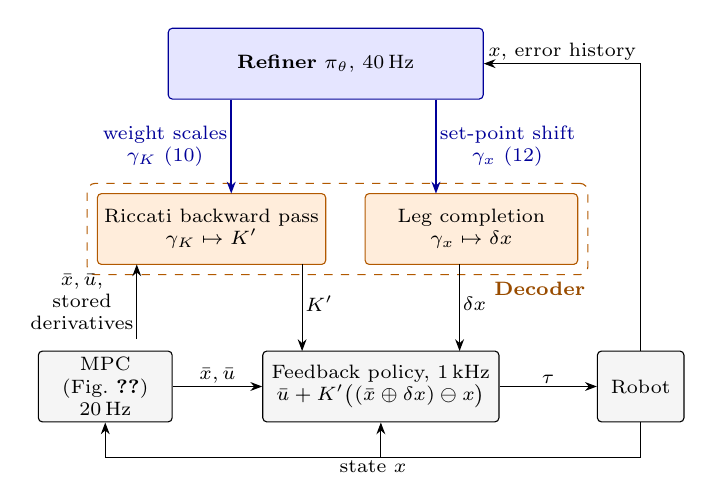
\begin{tikzpicture}[x=1mm, y=1mm, font=\scriptsize, >={Stealth[length=1.5mm]},
  blk/.style={draw, rounded corners=1.5pt, minimum height=9mm, align=center, inner sep=2pt, fill=black!4},
  res/.style={draw, rounded corners=1.5pt, minimum height=9mm, align=center, inner sep=2pt, fill=blue!10, draw=blue!60!black},
  dec/.style={draw, rounded corners=1.5pt, minimum height=9mm, align=center, inner sep=2pt, fill=orange!14, draw=orange!70!black},
  lab/.style={font=\scriptsize, align=center, inner sep=1pt}]
\node[blk, minimum width=17mm] (mpc) at (0,0) {MPC\\(Fig.~\ref{fig:base})\\20\,Hz};
\node[blk, minimum width=30mm] (fb) at (35,0) {Feedback policy, 1\,kHz\\$\ub+K'\big((\xb\oplus\delta x)\ominus x\big)$};
\node[blk, minimum width=11mm] (rob) at (68,0) {Robot};
\node[dec, minimum width=29mm] (bp) at (13.5,20) {Riccati backward pass\\$\gamma_K\mapsto K'$};
\node[dec, minimum width=27mm] (pr) at (46.5,20) {Leg completion\\$\gamma_x\mapsto\delta x$};
\node[draw=orange!70!black, dashed, rounded corners=3pt, inner sep=3.5pt, fit=(bp)(pr)] (decgrp) {};
\node[lab, text=orange!60!black, anchor=north east] at ($(decgrp.south east)+(0,-0.5)$) {\textbf{Decoder}};
\node[res, minimum width=40mm] (pol) at (28,41) {\textbf{Refiner} $\pi_\theta$, 40\,Hz};
\draw[->, blue!60!black, thick] (pol.south -| 16,0) -- node[lab, left, text=blue!60!black] {weight scales\\$\gamma_K$ (10)} (16,24.5);
\draw[->, blue!60!black, thick] (pol.south -| 42,0) -- node[lab, right, text=blue!60!black] {set-point shift\\$\gamma_x$ (12)} (42,24.5);
\draw[->] (4,6) -- node[lab, left] {$\xb,\ub$,\\stored\\derivatives} (4,15.5);
\draw[->] (25,15.5) -- node[lab, right, pos=0.45] {$K'$} (25,4.5);
\draw[->] (45,15.5) -- node[lab, right, pos=0.45] {$\delta x$} (45,4.5);
\draw[->] (mpc) -- node[lab, above] {$\xb,\ub$} (fb);
\draw[->] (fb) -- node[lab, above] {$\tau$} (rob);
\draw[->] (rob.south) -- (68,-9) -| node[lab, pos=0.25, below] {state $x$} (mpc.south);
\draw[->] (68,-9) -| (fb.south);
\draw[->] (rob.north) -- (68,41) -- node[lab, above] {$x$, error history} (pol.east);
\end{tikzpicture}
\caption{The refiner stack. The MPC of Fig.~\ref{fig:base} is treated as one block. The refiner outputs 22 numbers. The decoder turns them into a full gain matrix $K'$ by one backward pass of the solver and into a contact-consistent set-point shift $\delta x$.}
\label{fig:stack}
\end{figure}

\subsection{DDP backward recursion as a decoder for the gains}
The Riccati gains are a function of the cost \eqref{eq:costwb}, and we exploit this fact to obtain new gains.
The decoder does not change the cost of the MPC itself, i.e., every solve uses the original weights of \eqref{eq:costwb}, so the plan $\xb,\ub$ remains the same.
The decoder uses a copy $\ell'$ of the cost with scaled weights to recompute the gains.
Each scale multiplies one weight of \eqref{eq:costwb}:
\begin{align}
w'_j&=w_j\,e^{\gamma_j},\qquad j\in\{B,J,V,F,\tau_1,\dots,\tau_6\},\label{eq:scale}\\
w'_G&=w_G,\qquad w'_W=w_W.\label{eq:scaleG}
\end{align}
Here $\gamma_K=(\gamma_B,\gamma_J,\gamma_V,\gamma_F,\gamma_{\tau_1},\dots,\gamma_{\tau_6})$ contains four tracking scales (base orientation, joint posture, velocity and foot terms) and six torque scales (one per joint group).
Since multiplying all weights by a common factor only scales every $Q$ and $V$ in \eqref{eq:backward} and leaves $K'$ unchanged, we fix the CoM weight as the reference. As the CoM reference is the output of the LIPM model, we prefer the CoM to remain the main objective. Aside from that, we keep the cone penalty as it is.

The decoder then runs the backward pass once more along the current trajectory, with $\ell'$ in place of $\ell$.
Under the Gauss--Newton approximation used by the solver, the cost Hessian is linear in the weights, $\ell'_{xx}=\sum_c w'_c\,J_c\T W_cJ_c$ (and similarly for $\ell'_{ux},\ell'_{uu}$).
It is just a weighted sum of blocks the last solve has already computed; for the torque term it is a diagonal matrix with $w'_{\tau_g}$ on the joints of group $g$.
The dynamics Jacobians $f_x,f_u$ are stored as well, and torques at their bounds keep a zero gain, as in Box-FDDP.
The DDP recursion runs from the last node to the first:
\begin{align}
Q_{xx}&=\ell'_{xx}+f_x\T V^{+}_{xx}f_x,\nonumber\\
Q_{ux}&=\ell'_{ux}+f_u\T V^{+}_{xx}f_x,\nonumber\\
Q_{uu}&=\ell'_{uu}+f_u\T V^{+}_{xx}f_u,\nonumber\\
K'&=Q_{uu}^{-1}Q_{ux},\nonumber\\
V_{xx}&=Q_{xx}-Q_{ux}\T K',
\label{eq:backward}
\end{align}
where $V^{+}_{xx}$ is the value Hessian of the next node.

The backward pass runs only once to produce the gains along that trajectory.
Because \eqref{eq:backward} uses only Hessians and dynamics Jacobians and no cost gradients, it is the time-varying LQR around the trajectory with the new weights.
In this design, only the gains are replaced, so the decoded gains change the reaction but not the planned motion.

\begin{table}[t]
\caption{Latent representation $\gamma$ of the refiner}
\label{tab:latent}
\centering
\setlength{\tabcolsep}{3pt}
\resizebox{\columnwidth}{!}{%
\begin{tabular}{@{}llc@{}}
\toprule
Part & Content & Size\\
\midrule
$\gamma_K$, tracking & base orientation, posture, velocities, feet (CoM fixed) & 4\\
$\gamma_K$, torque & hip, knee, ankle; left and right leg & 6\\
$\gamma_x$ & base and swing-foot pose shifts; leg joints follow & 12\\
\midrule
\multicolumn{2}{@{}l}{Total, decoded into $K'\in\R^{12\times36}$ per node and $\delta x\in\R^{36}$} & 22\\
\bottomrule
\end{tabular}}
\end{table}

\subsection{Set-point shift}
The refiner outputs a shift $\delta b$ of the base pose and a shift $\delta s$ of the swing-foot pose, $\gamma_x=(\delta b,\delta s)$, both as 6-vectors in the tangent space.
The decoder turns them into a shift of the leg joints.
The set-point shift has the same layout as the state error,
\begin{equation}
\delta x=\begin{bmatrix}\delta b\\ \delta q_J\\ 0_{18}\end{bmatrix}\in\R^{36},
\label{eq:setpoint}
\end{equation}
with the base pose first ($\delta b\in\R^6$), then the twelve leg joints ($\delta q_J\in\R^{12}$), and a zero velocity part for the 18 base and joint velocities.
The shift is applied at the current time only and held until the refiner outputs the next $\gamma_x$, so it is an offset rather than a trajectory, and a zero velocity part is consistent with it.
To first order, a base shift $\delta b$ and a joint change $\delta q_{J,f}$ of leg $f$ move foot $f$ by
\begin{equation}
\delta p_f=J_{f,B}\,\delta b+J_{f,J}\,\delta q_{J,f},
\label{eq:footmotion}
\end{equation}
where $J_{f,B}$ and $J_{f,J}$ are the columns of the Jacobian of foot $f$ for the base and for the six joints of its leg.
A foot in contact must not move, and a swinging foot moves by $\delta s$:
\begin{equation}
\delta p_f=\begin{cases}0 & f\ \text{in contact},\\ \delta s & f\ \text{swinging}.\end{cases}
\label{eq:footshift}
\end{equation}
Away from a stretched knee, the $6\times6$ matrix $J_{f,J}$ is invertible, and solving \eqref{eq:footmotion} gives one rule for both legs,
\begin{equation}
\delta q_{J,f}=J_{f,J}^{-1}\big(\delta p_f-J_{f,B}\,\delta b\big).
\label{eq:legcompletion}
\end{equation}
A base shift therefore bends the legs without moving any foot, and $\delta s$ moves only the swing foot.
Together they span every set-point change that keeps the stance feet in place: of the 18 position coordinates of the base and legs, each stance foot removes six, leaving 12 in single support and the six of $\delta b$ in double support.
Unlike a projection onto the null space of the contact Jacobian, this reproduces the requested base shift exactly.

At liftoff and touchdown, the row of a foot in \eqref{eq:footshift} switches, and the joint set-point jumps by $J_{f,J}^{-1}\delta s$ unless $\delta s=0$.
We leave this to the policy, which observes the contact flags and the step phase and is penalized for $\|\delta s\|$ in double support and near touchdown.

Since the Riccati policy is the first-order expansion of the MPC solution \cite{fiacco1983sensitivity,dantec2022firstorder}, the torque $K'\delta x$ is, for a small shift, what the MPC with the refined weights would command if the robot were displaced by $-\delta x$: a learned bias on the state the controller sees.
It does not move the references of the MPC, so the robot settles where the pull of the MPC balances $K'\delta x$.
With $\zeta_i=x_i\ominus\xb_i$ and $A_i,B_i$ the dynamics Jacobians, the error evolves as
\begin{equation}
\zeta_{i+1}=(A_i-B_iK'_i)\,\zeta_i+B_iK'_i\,\delta x_i ,
\label{eq:cl}
\end{equation}
which stays bounded for a bounded shift if the time-varying closed loop is exponentially stable.

\subsection{Properties and limits}
\emph{Structured.} With positive weights, $Q_{uu}$ is positive definite and $K'$ is the optimal feedback of a valid local linear-quadratic problem.
The refiner can choose a poor cost, but it cannot produce a gain with flipped signs or a broken coupling between joints.
$K'$ is also consistent with the contacts because it is computed through the same contact-constrained dynamics.

\emph{Compact and meaningful.} The latent representation $\gamma$ has 22 numbers, each with a physical meaning that can be bounded and inspected.
The decoded gain depends smoothly on them.

\emph{Inexpensive.} The decoder reuses the cost-term and dynamics Jacobians stored by the last MPC solve, so it evaluates no model derivative: it forms a weighted sum and runs one Riccati recursion over 20 nodes.
With $\gamma_K=0$, it reproduces the gains of the MPC exactly.

\emph{Bounded.} This structure is not a safety guarantee: the gains come from a 0.5\,s horizon and stabilize the model rather than the robot, and extreme weight ratios give high gains that become unstable with actuation delay.
Each scale therefore has a calibrated bound, since the gains do not respond evenly to the weights, and $\gamma$ is rate-limited, since a fast-varying gain can destabilize a loop even when every frozen value is stabilizing.
A safety check is left for future work: before $\gamma$ is applied, the closed loop \eqref{eq:cl} could be rolled out over the horizon and $\gamma$ shrunk if the predicted error or torques leave their bounds, as a predictive safety filter does \cite{wabersich2021psf,ames2019cbf,brunke2022safe}.

\emph{Limits.} The decoder only reaches gains that are optimal for some cost on the model's dynamics, so if those dynamics are wrong, the best gain may lie outside this family.
The refiner also cannot change the footsteps or the contact schedule, so disturbances that need a different step remain the job of the gait generator.

\subsection{Learning for robustness}
The refiner observes the state, a short history of tracking errors and torques, the contact flags and step phase, the velocity command and its own previous output.
From the history it can recognize the situation, such as a heavier robot or a softer floor, and pick weights for it rather than learning one compromise setting.
It is trained with PPO \cite{schulman2017ppo} in simulation under the uncertainties it should withstand: pushes, mass and CoM offsets, friction, contact stiffness and actuation delay.
The reward combines velocity tracking and staying upright with penalties on the size and rate of $\gamma$, on joint torques, on a center of pressure (CoP) near the sole edge, on a tilted stance foot and on a swing-foot shift $\delta s$ in double support or near touchdown.
Since the MPC and the decoder are part of the environment, no derivative of the solver is needed.

\section{Preliminary Results: Base Controller}
\label{sec:results}

The refiner has not been trained yet, so this section reports the base controller alone.
It sets the baseline and shows what the refiner will have to correct.

\subsection{Setup}
The controller is implemented in C++ as an mc\_rtc plugin and runs on the HRP-5P model (104\,kg) in mc\_mujoco \cite{singh2022mcmujoco}, a MuJoCo \cite{todorov2012mujoco} interface, with a 1\,ms step and torque control.
Both solvers run inside the control step, which is acceptable in simulation but not yet real time.
All results come from the same laptop (Intel Core Ultra 9 185H) and one version of the controller: the robustness tests run several cases in parallel, and the walking tests and timings run one case at a time.
On one machine a case is deterministic, but whole sweeps have differed by one or two pushes between repeats, which we treat as noise.
A run fails when a joint stays at its torque limit for more than 50\,ms, which triggers a safety stop, or when the base drops below 0.6\,m.
A push is a 0.1\,s force on the base, given as its impulse.

\subsection{Walking}
Straight walking reaches 101 to 104\,\% of the commanded speed from 0.4 to 0.5\,m/s, but only 90\,\% from 0.1 to 0.3\,m/s.
Turning in place up to 0.3\,rad/s, walking at 0.5\,m/s while turning at 0.3\,rad/s and walking backward all run without a stop or a fall, as do all 16 cases of this test.
At 0.5\,m/s, the median whole-body solve takes 5.8\,ms (three iterations) of its 50\,ms period, an IS-MPC tick 1.5\,ms and a pre-optimization 8.7\,ms.
Warm-started solves stop at ten iterations; only the cold first solve takes longer (up to 85\,ms).

\begin{table}[t]
\caption{Failures and push recovery of the base controller}
\label{tab:robust}
\centering
\setlength{\tabcolsep}{3pt}
\resizebox{\columnwidth}{!}{%
\begin{tabular}{@{}lcccc@{}}
\toprule
Controller & Random & Restarts & Pushes, & Pushes,\\
 & (falls) & (falls) & one step & full stride\\
\midrule
Open-loop gait, FDDP, 10\,Hz & 1/28 & 0/12 & 28/48 & 50/104\\
+ step adaptation & 0/28 & 0/12 & 30/48 & 57/104\\
+ Box-FDDP within the torque limits & 0/28 & 0/12 & 32/48 & 64/104\\
+ measured ZMP support & 0/28 & 0/12 & 35/48 & 66/104\\
+ whole-body MPC at 20\,Hz (ours) & 0/28 & 0/12 & \textbf{37/48} & \textbf{80/104}\\
\midrule
ismpc\_walking \cite{mc_ismpcwalking} (position control) & 1/28 & 0/12 & 36/48 & 70/104\\
\bottomrule
\multicolumn{5}{@{}l}{Random: 40\,s schedules of random commands. Restarts: walking again after a}\\
\multicolumn{5}{@{}l}{stop. Pushes: 30 and 40\,N\,s in four directions while walking at 0.25\,m/s, at six}\\
\multicolumn{5}{@{}l}{instants of one step or at 13 instants 0.2\,s apart over a full stride. Recovered}\\
\multicolumn{5}{@{}l}{pushes of ismpc\_walking include 3 and 7 in which it stops walking.}
\end{tabular}}
\end{table}

\subsection{Robustness}
Table~\ref{tab:robust} tests every row on the same 28 random command schedules, 12 restarts from standing and two push sets.
Step adaptation removes the only fall on the random schedules and adds 2 one-step and 7 full-stride pushes; no variant falls on the restarts.
Box-FDDP adds 2 and 7 more; in a separate sweep, the gain came from the solver, since bounding the torques at the real limits changed nothing measurable and bounding them at 90\,\% of the limits lost five pushes.
Centering the ZMP limits on the measured feet adds 3 and 2.

The one-step set covers only one stance phase of our 0.8\,s steps and turned out to favor it: over a full stride, the same controller recovers only 66 of 104 pushes.
Running the whole-body MPC at 20\,Hz instead of 10\,Hz, with the same 0.5\,s horizon in 20 knots of 25\,ms, raises this to 80 of 104 (20 newly recovered, 6 lost) and the one-step set to 37 of 48, without any fall on the schedules or restarts.
In a separate sweep, the gain came from the rate, not the knots: 25\,ms knots at 10\,Hz recovered only 53 of 104.
The open-source ismpc\_walking controller \cite{mc_ismpcwalking}, run on the same machine and scenarios with position control, recovers 36 of 48 and 70 of 104 pushes, ten of them by stopping; with its default gait, it walks at up to 0.28\,m/s.
It runs in real time, so its results vary more between runs (79 of 104 in an earlier run).
All forward and all but one backward pushes are recovered; 23 of our 24 failures come from sideways pushes.

\subsection{What the refiner has to correct}
The results point to three weaknesses, each of which maps to a part of $\gamma$, and to one that lies outside its reach.

\emph{Execution after a strong push.} After a 40\,N\,s sideways push, the gait generator plans the recovery step and the foot lands about 0.3\,s later with the DCM inside it.
At 10\,Hz, the robot still failed during the execution.
The stance foot slid by 4.6\,cm under the large lateral force, the swing foot lagged its moving target by up to 8.5\,cm and landed with 3\,kN, and a joint then stayed at its torque limit.
Over the full stride, 25 of the 38 failures at 10\,Hz happened in the execution before any recovery step, with a joint, mostly an ankle, at its torque limit about 0.17\,s after the push.
The wrench cone is only a penalty in the OCP, and the gains are tuned for normal walking.
Fixed caps on the ankle torques in the OCP did not help (three to seven pushes fewer).
Running the MPC at 20\,Hz leaves only 1 of 24 failures of this kind: a feedback policy refreshed twice as often recovers 14 more pushes, which shows how much depends on the policy between two solves.
Higher torque weights on the leg in stance and a higher foot weight during the swing are the kind of change the refiner can make in that situation, without the cost of solving more often.

\emph{Tracking the LIPM.} The CoM path of the LIPM fits the robot's sideways motion well but explains only 39\,\% of its forward CoM acceleration.
Tracking it stiffly forces the robot away from its own dynamics: raising the forward and sideways CoM weights to 5000 made seven of eight random schedules fail.
A set-point shift can counter the systematic part of this mismatch with a steady bias, without stiffening the tracking.

\emph{No single set of weights.} In earlier sweeps without step adaptation, every weight setting failed on about 20\,\% of fresh random schedules, and the same schedules failed under all of them.
Weight tuning had reached its limit, which is the motivation for weights that change with the situation.

\emph{Recovery steps that fall short.} At 20\,Hz, 23 of the 24 failures come 0.8\,s or more after the push, after a median of two recovery steps, and only two of them ever place a foot beyond the measured DCM, against 56 of the 80 recovered pushes (median margin 29\,mm).
These failures need a longer or earlier step, which is the job of the gait generator and outside the reach of the refiner.

\section{Conclusion}
We built a torque-controlled walking controller for HRP-5P that couples an IS-MPC gait generator, which solves footstep positions and timing jointly and adapts the swing step to the measured DCM, with a whole-body MPC of the legs solved by Box-FDDP at 20\,Hz within the torque limits.
In simulation, the robot walks at up to 0.5\,m/s, turns and walks backward with a median whole-body solve of 5.8\,ms, does not fall on random schedules or restarts, and recovers 80 of 104 pushes over a full stride, on par with an open-source IS-MPC walker.
Most remaining failures are sideways pushes whose recovery steps land short of the DCM.

Since a whole-body MPC is optimal only for its model, we proposed a control policy refiner that modifies the gain and set-point of its feedback policy through 22 cost-weight scales and set-point shifts, decoded by one backward pass of the solver, which keeps learning structured and low-dimensional.
Replanning twice as often recovered 14 more pushes, which shows how much depends on the feedback between solves; training the refiner is our next step.

% slightly smaller reference list (small deviation from the IEEE template, to stay within 6 pages)
\begingroup
\raggedright
\renewcommand{\footnotesize}{\fontsize{7.5}{8.6}\selectfont}
\bibliographystyle{IEEEtran}
\bibliography{refs}
\endgroup

\end{document}
